\documentclass[12pt, a4paper]{article}
\usepackage[utf8]{inputenc} %codification of the document

\usepackage{authblk}% This one is for adding affiliation of an author \affil command

%--------------------------
%Package for comment
\usepackage{comment}
%-------------------------------
%Package for coloring text
%\usepackage{xcolor}

%---------------------------------

% Package for math

\usepackage{amsmath}
%------------------------------------------

% Package for images

\usepackage{graphicx}


%------------------------------------------

% Package for coding

\usepackage{listings}


%------------------------------------------
% Package for algorithms

\usepackage[ruled,vlined]{algorithm2e}


%------------------------------------------

%%For coloring and linking the reference and url. 
\usepackage{hyperref}
\hypersetup{
    colorlinks=true,
    linkcolor=blue,
    filecolor=magenta,      
    urlcolor=blue,
    pdftitle={Sharelatex Example},
    bookmarks=true,
    pdfpagemode=FullScreen,
}
%%---------------------------------
%% A macro is a shorthand for a more complicated sequence of commands. Later in the text, the macro can be used instead of those sequence of commands. 

\newcommand {\pr}{\textit{Projection,}$\pi$}
\newcommand {\se}{\textit{Selection,} $\sigma$}
\newcommand {\cp}{\textit{Cartesian product,}$\times$}
\newcommand {\un} {\textit{Union,}$\cup$}
\newcommand {\di}{\textit{Set difference,}$-$}
\newcommand {\re}{\textit{Rename,}$\rho$}

%----------------------------

%\begin{center}
%A thesis submitted to the Technical Faculty of IT and Design at Aalborg University (AAU) and the Department of Service and Information System Engineering at Universitat Politècnica de Catalunya (UPC), in partial fulfillment of the requirements within the scope of the IT4BI-DC programme for the joint Ph.D. degree in Computer Science. The thesis is not submitted to any other organization at the same time.
%\end{center}


%-------------------------


%-------------------------------
\begin{document}

%\begin{titlepage}

\begin{figure}
	\centering
	\begin{minipage}[b]{0.15\textwidth}
		
\includegraphics[width=1\textwidth]{images/cu}
		%\caption{Black Image}
	\end{minipage} \hfill
	\end{figure}
	
\noindent%
  \begin{tabular}{@{}p{\textwidth}@{}}
    \hline
    \hline
    \vspace{0.2cm}
    \begin{center}
    \Huge{\textbf{
    CU VIRTUAL CLASSROOM % insert your title here
    }}
    \end{center}
    \vspace{0.2cm}\\
    \hline
    \hline
  \end{tabular}
  \vspace{4 cm}

\begin{center}
    {\large
      Database Project Report %Insert document type (e.g., Project Report)
    }\\
    \vspace{0.2cm}
    {\Large
      Group-06 % Insert group number
      
    }
  \end{center}
  \vfill
  
  \begin{center}
  Report submitted February, 2023
  \end{center}
	\vfill
A project submitted to Dr. Rudra Pratap Deb Nath, Associate Professor, Department of Computer Science and Engineering, Chittagong University (CU) in partial fulfillment of the requirements for the Database Systems Lab course. The project is not submitted to any other organization at the same time. 

\end{titlepage}
\clearpage
%%%%% Details of student
%-------------------------
%Fill up the table with your group information
%----------------------------

\begin{table}[t]
\caption{Details of Group-01}% insert your group number 
\resizebox{\textwidth}{!}{%
\begin{tabular}{|l|l|l|l|l|}
\hline
Roll Id & Name & Sigature & Date & Supervisor Approval \\ \hline
        &      &          &      &                     \\ \hline
        &      &          &      &                     \\ \hline
        &      &          &      &                     \\ \hline
        &      &          &      &                     \\ \hline
        &      &          &      &                     \\ \hline
        &      &          &      &                     \\ \hline
\end{tabular}%
}
\end{table}
\clearpage






%-------------------------

% Showing contents as an Index
\setcounter{secnumdepth}{5}
\setcounter{tocdepth}{5}
\tableofcontents
\listoffigures

\listoftables
\lstlistoflistings
%-----------------------




%abstract.tex

\begin{abstract}
The Virtual Classroom Android App project is aimed to develop a database application system by applying the theories, methodologies, tools, and technologies learned in Database Management System course. The motivation behind this project is to provide an alternative solution to traditional physical classrooms. This project addresses the need for a virtual classroom environment for students where they can join one classroom, receive class updates, schedule transportation,access class resources and upcoming events, and view semester information such as course lists, syllabus etc . The current solutions have limitations in terms of flexibility and scheduling. The approach used to fill this gap is the implementation of a virtual classroom android app using the system development process that includes the requirement
gathering and analysis, database modelling, system architecture, implementation and validation. The solution provided by this system is a virtual classroom android app that allows students to join one virtual classroom, receive class updates, schedule transportation, access class resources, and upcoming events, and view semester information such as course lists, syllabus, etc. The solution will be evaluated based on its usability and effectiveness. The significance of this project is that
it allows students to continue their education from anywhere, at any time. However, the limitation of this project is that it's for the android platform only, and for future work, we can enhance the app by adding more features and making it available for other platforms as well.
\end{abstract}
\clearpage
% Maintain the consistency.
% Maintain a good writing flow. 

\section{Introduction}\label{sec:introduction}
This document is a documentation of the Virtual Classroom Android App project. The objective of this project is to develop a database application system by applying the theories, methodologies, tools, and technologies learned in Database Management System course]. The app aims to provide a virtual classroom environment for students where they can join in one classroom,
receive class updates, schedule transportation, access class resources, and upcoming events, and view semester information such as course lists, syllabus etc.  


\subsection{Background and Motivation}\label{subsec:bm}

In today's world, online learning has become a popular and necessary approach due to the  COVID-19 pandemic and social distancing norms. The current state of the problem is that traditional physical classrooms are not feasible, and there is a need for an alternative solution. The virtual classroom app aims to address this problem by providing a virtual classroom environment for students. The significance of this solution is that it allows students to continue their education from anywhere, at any time, and it also allows for flexibility in scheduling and learning.

\subsection{Problem Statement}\label{subsec:ps} 
This project aims to address the need for an alternative solution to traditional physical classrooms. The project aims to create a virtual classroom app that allows students to join one classroom, receive class updates, schedule transportation, access class resources, and upcoming events, and view semester information such as course lists, syllabus, etc. The entities in this problem include students, classes, resources, events, and semesters. The relationships between these entities include one-to-many and many-to-many.


\subsection{System Definition}\label{subsec:sd} 

The Virtual Classroom Android App is a computerized system that allows students to join the virtual classroom, receive class updates, schedule transportation, access class resources, and upcoming events, and view semester information such as course lists, syllabus, etc. The system is designed to be easy to use and understand for students, and it allows for flexibility in scheduling and learning.


\subsection{System Development Process}\label{subsec:sdp}

To development this  system ,  we follow the following steps:
\begin{enumerate}
\item Requirement analysis
	\begin{itemize}
		\item[-] In this step, the project team gathers and analyzes the requirements for the database, including the entities, attributes, and relationships needed. The output of this step is a clear understanding of the requirements for the database.
	\end{itemize}

\item Mapping onto a conceptual model (conceptual design)
     \begin{itemize}
     	\item[-] In this step, the project team creates a conceptual model of the database using the ER model. This step includes creating an Entity-Relationship (ER) diagram, which represents the relationships between the entities in the database. The output of this step is a well-designed conceptual model of the database.
     	
     \end{itemize}
     
\item Mapping onto a data model (logical design)
	\begin{itemize}
     	\item[-] In this step, the project team maps the conceptual model onto a logical data model, such as the relational or object model. This step includes creating a logical design of the database, including tables, attributes, and relationships. The output of this step is a well-designed logical data model of the database.
     \end{itemize}
     
\item Normalization
\begin{itemize}
     	\item[-] In this step, the project team normalizes the logical data model to ensure that it is in the 3rd normal form (3NF) and is free from data redundancy and inconsistencies. The output of this step is a normalized database design.
     \end{itemize}
\item System Architecture
\begin{itemize}
     	\item[-] In this step, the project team designs the overall architecture of the system, including the user interface and database design. This step includes creating wireframes and mockups of the app, and determining the overall structure of the app. The output of this step is a detailed system architecture.
     \end{itemize}
     
\item Realization and Implementation (physical design) 
\begin{itemize}
     	\item[-] In this step, the project team codes and develops the database, including the front-end and back-end. This step includes writing code for the app, testing the app, and debugging any errors. The output of this step is a fully functional database.
     \end{itemize}   
    
    
    Each step of the database design process will be a separate section of this document, and the output of each step will be used as the input for the next step.
\end{enumerate}


\begin{figure}[h]

\centering
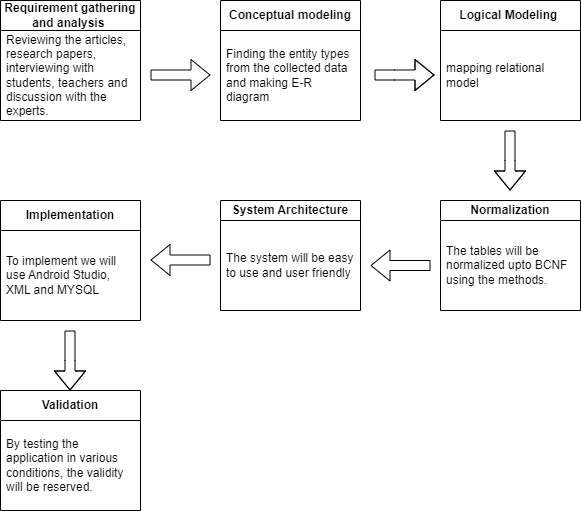
\includegraphics[scale=.5]{sys}

\caption{System Development Process }
\end{figure}


\subsection{Organization} The organization of this document is as follows:

Section~\ref{sec:introduction} gives an overview of the project, including the motivation, problem statement, system definition, and system development process.

Section~\ref{sec:projectmanagement} describes the project management, including the organization of resources, roles of team members, and tools used.

Section~\ref{sec:rga} describes the requirement gathering and analysis process in detail.

Section~\ref{sec:cm} describes the process of creating the conceptual model and ER diagram for the database.

Section~\ref{sec:lm} describes the process of creating the logical data model and mapping the conceptual model onto it.

Section~\ref{sec:norm} describes the process of normalizing the database design.

Section~\ref{sec:sa} describes the system architecture in detail.

Section~\ref{sec:imp} describes the process of coding and implementing the database and android app.

Section~\ref{sec:val} describes the process of testing and validating the database and android app.

Finally, the conclusion and the pointers to the future work are outlined in Section~\ref{sec:cfw}.




\clearpage
\section{Project Management}\label{sec:projectmanagement}
This project aims to develop a virtual classroom which primarily meets the needs of students of CSE CU. 


All project documentation can be found at:
Trello Link: \href{https://trello.com/b/JfOtRvVs/project-idea}{trello} 

Github Link:\href{https://github.com/Sharif37/CU-Virtual-Classroom-}{github} 




The roles of each members:
\begin{enumerate}


\item Kazi Omar Sharif(20701015): Developed the project plan. Recruited necessary stuffs to proceed with the project. Determined the methodology that will be used on this project.Created a  Trello account and a Github account. Hosted a Zoom meeting.Assigned tasks to project team members.Contributed in releasing the press release.Contributed in  Database Project Report documentation. 

\item Mohammad Fazly Rabby(20701070): Solved project objectives. Recruited necessary information that needed for the project. Contributed in releasing the press release. 

\item Saiyed Mohammad Hasan(20701023): Constantly working with the users to establish and meet the needs. Helped in writing the press release.  

\item Priya Barua(20701041):Carefully detecting the errors while executing the project. Contributed in releasing the press release. 
\end{enumerate}
\clearpage
\section{Requirement Gathering and analysis}\label{sec:rga}
To gather the requirements for the Virtual Classroom Android App project, several methods were used, including documentation, interviewing, survey, and discussion.
\begin{itemize}
\item Documentation: The project team reviewed existing literature and documents related to virtual classrooms, including articles, research papers, and other relevant resources, to gather an understanding of the current state of the problem and existing solutions.

\item Interviewing: The project team conducted interviews with potential users of the app, such as students, teachers, and administrators, to gather their views on the current problems faced in virtual classrooms and their requirements for an ideal virtual classroom app.


\item Discussion: The project team held internal and external discussions with experts in the field of virtual classrooms, to gather their views on the current problems faced in virtual classrooms and their requirements for an ideal virtual classroom app.
\end{itemize}
The stack-holders of the system are students.

\textbf{Functional requirements:}

\begin{itemize}
\item Students  should be able to join a virtual classroom
\item Students  should be able to see class updates
\item Students  should be able to see the schedule for transports
\item Students  should be able to see class resources and upcoming events
\item Students should be able to see semester information including course list, syllabus and teachers list
\item Students should be able to communicate through the app

\end{itemize}
\textbf{Non-functional requirements:}

\begin{itemize}
\item The app should be user-friendly and easy to navigate
\item The app should have high availability and should be accessible at all times
\item The app should have a high level of security to protect user data
\item The app should be able to handle large amounts of data
\item The app should be compatible with different devices and screen sizes
\item The app should be responsive and should load quickly

\end{itemize}



\clearpage
\section{Conceptual Modelling}\label{sec:cm}

\begin{figure}[h]

\centering
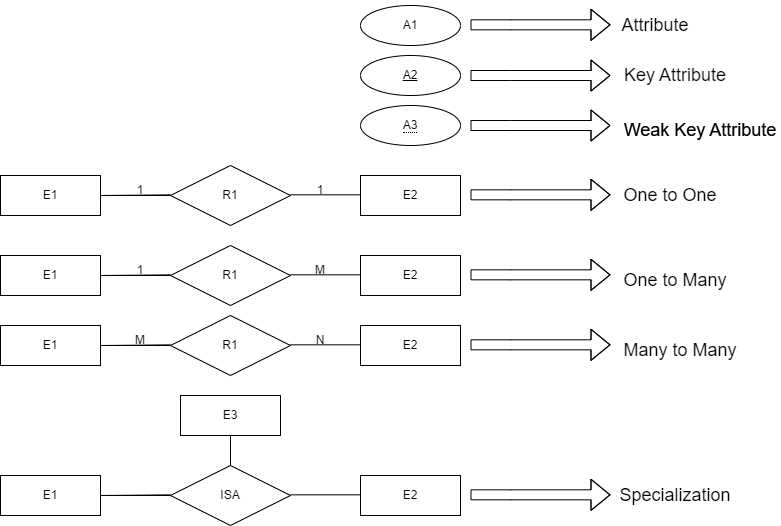
\includegraphics[scale=.5]{info1u}

\caption{Legends}
\end{figure}

\clearpage

\begin{figure}[h]

\centering
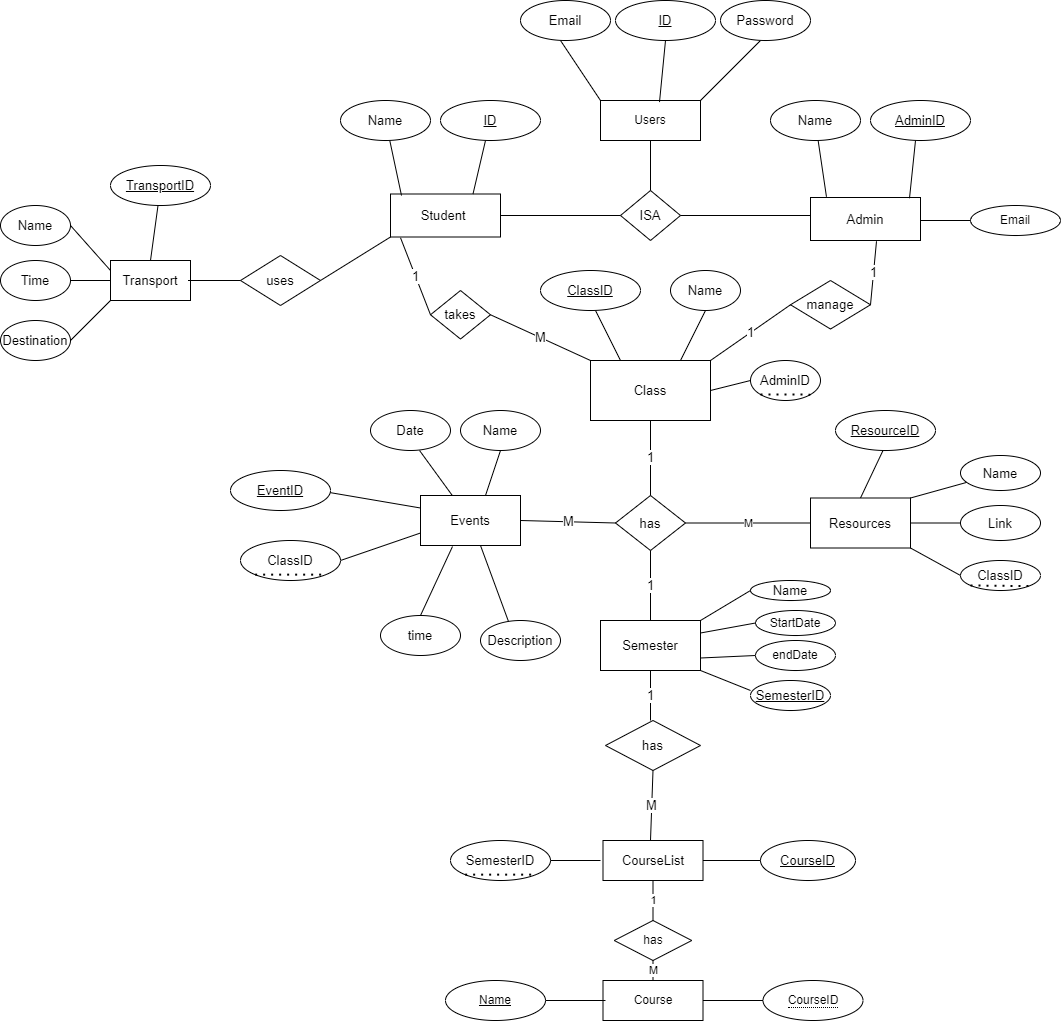
\includegraphics[scale=.4]{er2}

\caption{The E-R diagram for virtual classroom }
\end{figure}
 
 

The E-R diagram for the Virtual Classroom Android App project is as follows:

\begin{itemize}

\item The entity types in the diagram are users , Student, Class, admin , Semester, Course, Resource, Event, and Transport.

\item The relationships between the entities are:
    \begin{itemize}
   \item  Student is takes in one class (Many-to-one relationship)
   \item Class has one Admin (One-to-One relationship)
   \item Class has one Semester (One-to-One relationship)
   \item Semester includes one or more courses (One-to-Many relationship)
   \item Class has one or more resources (One-to-Many relationship)
   \item Class has one or more upcoming events (One-to-Many relationship)
   \item students use transports(Many to Many relationship) 
   \item semester has courseList (One-to-Many relationship)
    \end{itemize}
  \item The attributes of each entity are:
   \begin{itemize}
   \item Users: Email,ID,Password 
   \item Student: ID, Name 
   \item Class: ClassID, Name, AdminID ,SemesterID
   \item Admin: ID, Name, Email 
   \item Semester: semesterID, Name, Start Date, End Date 

  \item Resource: ResourceID, Name,Link, ClassID
  \item Event: EventID, Name, Date, ClassID, Description,time 
  \item Transport: TransportID, Name, time , Destination
  \item courseList: courseID,semesterID 
  
  
   \end{itemize}

\end{itemize}

The E-R diagram was created by first identifying the key entities in the system, which include Students, Classes, ClassRepresentative, Semester, Course, Resource, Event, and Transport. The relationships between these entities were then identified, such as a student being enrolled in one or more classes, and a class having one ClassRepresentative. The attributes of each entity were also identified, such as a student having an ID, name, email, phone number, and profile picture. The E-R diagram was then created by visually representing these entities, relationships, and attributes using the standard ER notation.

\section{Logical Modelling}\label{sec:lm}

A relational model is a method of organizing data in a database using a collection of tables with rows and columns. Each table represents a specific entity or relationship in the data, and the columns represent the attributes or properties of that entity or relationship.

To convert an E-R diagram to a relational model, we can start by identifying the entities in the E-R diagram and creating a table for each one. The columns of the table will correspond to the attributes of the entity. We then identify the relationships between the entities and create additional tables to represent these relationships. The columns of these tables will correspond to the foreign keys, linking the rows of the related tables together. In our case, we have multiple entities such as users, students, class, admin, semester, course, resource, event, and transport. Each entity is represented by a table. The relationships between the entities are represented as foreign keys in the table. For example, the Student table has a foreign key to the Class table, representing the many-to-many relationship between students and classes. Similarly, the Class table has a foreign key to the Semester table, representing the one-to-one relationship between a class and a semester.

\clearpage
\section{Normalization}\label{sec:norm}

 The functional dependencies for each relation in the normalized relational model:

Relation 1: Users\\


Email $\rightarrow$ ID, Password\\

 ID $\rightarrow$ Email, Password\\

Relation 2: Student\\


ID $\rightarrow$ Name\\

Relation 3: Class\\


ClassID $\rightarrow$ Name, AdminID, SemesterID\\

Relation 4: Admin\\


ID $\rightarrow$ Name, Email\\


Relation 5: Semester\\

SemesterID $\rightarrow$ Name, Start Date, End Date\\

Relation 6: Resource\\


ResourceID $\rightarrow$ Name, Link\\

ClassID $\rightarrow$ Name \\

Relation 7: Event\\


EventID $\rightarrow$ Name, Date, Description, Time\\

ClassID $\rightarrow$ Name \\


Relation 8: Transport \\

TransportID $\rightarrow$ Name, Time, Destination \\


Relation 9: Course\\

CourseID $\rightarrow$ Name \\


Relation 10: CourseList\\

CourseID $\rightarrow$ Name \\

SemesterID $\rightarrow$ Name \\

These relations are in 3NF, as all non-key attributes are functionally dependent on the primary key and there are no transitive dependencies.\\




\clearpage
\section{System Architecture}\label{sec:sa}
Describe the architecture of your system using a figure: Describe how each component of the architecture communicate. 
\clearpage
\section{Implementation}\label{sec:imp}
Give some code snippet of each component you outlined in your System architecture. Some DDL query example. Use the listing environment for writing code. 
Listing~\ref{list:sql} shows an SQL query. 

\begin{lstlisting}[caption={A SQL query example}, label=list:sql, captionpos=b,
           backgroundcolor=\color{white},
           language=SQL,
           breaklines=true,
           frame=single,
           showspaces=false,
           basicstyle=\ttfamily,
           numbers=left,
           numberstyle=\tiny,
           rulecolor=\color{red},
           keywordstyle=\color{blue},
           commentstyle=\color{gray}
        ]
select distinct name
from instructor
where salary > some( select salary
			from instructor
			where dept_name='CSE');
\end{lstlisting}
\clearpage

\section{Validation} \label{sec:val}
Show that users are satisfied with your product. 
You can also give a user manual here describing how to use your system (process of completion of different tasks using your system )
You can use some matrices (time, cost, resource etc.) to compare your system with the previous system. 
\clearpage
\section{Software Deployment}\label{sec:sd}
Describe how to install and configure your system so that a non-technical user can use your system. 

\clearpage
\section{Conclusion and Future Work}\label{sec:cfw}
Write the conclusion of your project: what was the problem? what the developed solution offers, Significance of the project, limitations of the project and future work. 
\clearpage












\section{Bibliography} 
\label{sec:bibliography}
To add bibliography in your document, use the following steps:
\begin{enumerate}
\item First create a .bib file in the same directory where your .tex file is (in our case, the file name is references.bib). Also place the bibliography style file in the same directory. In our case, we are using the ios1.bst style file. We include the following commands in the .tex file for the style file and bib file: \\
 \texttt{\textbackslash bibliographystyle\{ios1\}} \\
\texttt{\textbackslash bibliography\{references\}} 
\item Import the BibTeX of your book or paper from Google Scholar or other sources into your .bib file. An example of BibTex is shown in Listings~\ref{list:bibtex}.  

\begin{lstlisting}[caption={A BibTeX example}, label=list:bibtex, captionpos=b,
           backgroundcolor=\color{white},
           language=SQL,
           breaklines=true,
           frame=single,
           showspaces=false,
           basicstyle=\ttfamily,
           numbers=left,
           numberstyle=\tiny,
           rulecolor=\color{red},
           commentstyle=\color{gray}
        ]
@article{kopka1995guide,
  title={A Guide to $\{$$\backslash$LaTeX$\}$--Document},
  author={Kopka, H and Daly, PW},
  year={1995},
  publisher={Citeseer}
}
\end{lstlisting}

\item Then, use the name of the BibTex (in Listing~\ref{list:bibtex}, the name is kopka1995guide) in the text of your .tex document where you want to refer it.

\item After saving your .tex document, execute the PDFLaTeX option one time; then execute the BibTeX option; then again execute the PDFLaTeX option for twice; finally, execute the QuickBuild option. Now your document refer the corresponding book or paper. 
\end{enumerate}

\bibliographystyle{ios1}

\bibliographystyle{plain}
\bibliography{references}


\end{document}